\documentclass[11pt]{article}
\usepackage{amssymb}
\usepackage{amsthm}
\usepackage{enumitem}
\usepackage{physics,amsmath}
\usepackage{bm}
\usepackage{adjustbox}
\usepackage{mathrsfs}
\usepackage{graphicx}
\usepackage{siunitx}
\usepackage[mathscr]{euscript}

\title{\textbf{Solved selected problems of Classical Mechanics - Gregory}}
\author{Franco Zacco}
\date{}

\addtolength{\topmargin}{-3cm}
\addtolength{\textheight}{3cm}

\newcommand{\hatr}{\bm{\hat{r}}}
\newcommand{\hatx}{\bm{\hat{x}}}
\newcommand{\haty}{\bm{\hat{y}}}
\newcommand{\hatz}{\bm{\hat{z}}}
\newcommand{\hatth}{\bm{\hat{\theta}}}
\newcommand{\hatphi}{\bm{\hat{\phi}}}
\newcommand{\hatrho}{\bm{\hat{\rho}}}
\newcommand{\ngrad}[1]{\text{grad}_{\bm{#1}}}

\theoremstyle{definition}
\newtheorem*{solution*}{Solution}
\renewcommand*{\proofname}{\bf{Solution}}

\begin{document}
\maketitle
\thispagestyle{empty}

\section*{Chapter 15 - The general theory of small oscillations}

\begin{proof}{\textbf{15.3}}
    The system looks like the following
    \begin{center}
        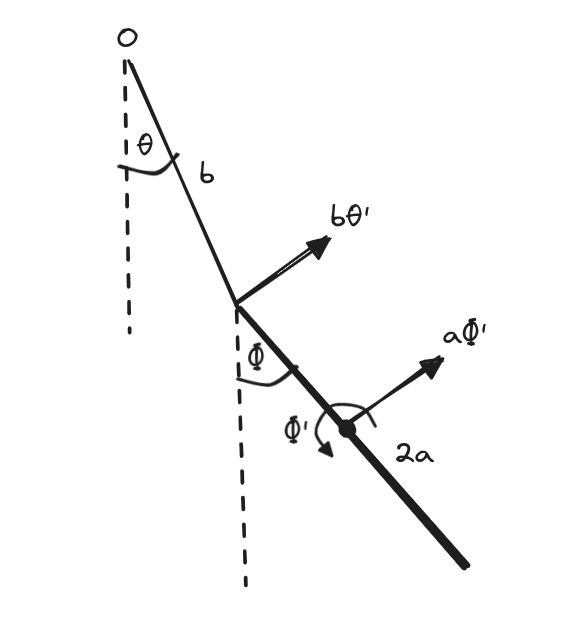
\includegraphics[scale=0.4]{ch15-3.png}
    \end{center}
    Then the kinetic energy of the system is given by
    \begin{align*}
        T &= \frac{1}{2}m(b\bm{\dot\theta} + a\bm{\dot\phi})^2
        + \frac{1}{2}\left(\frac{1}{3}ma^2\right)\dot\phi^2\\
        &= \frac{1}{2}m\left((b\dot\theta)^2
        + 2(b\dot\theta)(a\dot\phi)\cos(\theta-\phi) + (a\dot\phi)^2\right)
        + \frac{1}{2}\left(\frac{1}{3}ma^2\right)\dot\phi^2
    \end{align*}
    On the other hand, the potential energy is given by
    \begin{align*}
        V = mg b(1 - \cos\theta) + mga(1 - \cos\phi)
    \end{align*}
    But for small oscillations about $\theta = \phi = 0$ we can approximate
    the equations for $T$ and $V$ as follows
    \begin{align*}
        T &= \frac{1}{2}m\left(b^2\dot\theta^2
        + 2(b\dot\theta)(a\dot\phi)
        + \frac{4}{3}a^2\dot\phi^2\right)\\
        V &= \frac{1}{2}mg(b\theta^2 + a\phi^2)
    \end{align*}
    Then Lagrange's equations of the system using the linearized
    $T$ and $V$ are given by
    \begin{align*}
        \derivative{}{t}\partialderivative{T}{\dot\theta}
        - \partialderivative{T}{\theta} &= - \partialderivative{V}{\theta}\\
        mb^2 \ddot\theta + mba\ddot\phi &= - mgb\theta\\
        b \ddot\theta + a\ddot\phi &= - g\theta
    \end{align*}
    And
    \begin{align*}
        \derivative{}{t}\partialderivative{T}{\dot\phi}
        - \partialderivative{T}{\phi} &= - \partialderivative{V}{\phi}\\
        mba\ddot\theta + ma^2 \ddot\phi + \frac{1}{3} ma^2 \ddot\phi
        &= - mga\phi\\
        b \ddot\theta + \frac{4}{3}a\ddot\phi &= - g\phi
    \end{align*}
    Also, the $\bm{V}$-matrix and the $\bm{T}$-matrix are 
    \begin{align*}
        \bm{V} = \frac{1}{2}mg\begin{pmatrix}
            b  & 0\\
            0 & a
        \end{pmatrix}\quad\quad
        \bm{T} = \frac{1}{2}m\begin{pmatrix}
            b^2  & ba\\
            ba & \frac{4}{3}a^2
        \end{pmatrix}
    \end{align*}
    Now let $b = 4a/5$ then the determinant equation is given by
    \begin{align*}
        \det\begin{bmatrix}
            \frac{1}{2}mga \begin{pmatrix}
                4/5 & 0\\
                0 & 1
            \end{pmatrix}
            - \frac{1}{2}ma^2\omega^2 \begin{pmatrix}
                16/25 & 4/5\\
                4/5 & 4/3
            \end{pmatrix}
        \end{bmatrix} &= 0\\
        \det\begin{bmatrix}
            g \begin{pmatrix}
                4/5 & 0\\
                0 & 1
            \end{pmatrix}
            - a\omega^2 \begin{pmatrix}
                16/25 & 4/5\\
                4/5 & 4/3
            \end{pmatrix}
        \end{bmatrix} &= 0\\
        \begin{vmatrix}
            \frac{4}{5}g -\frac{16}{25}a\omega^2 & -\frac{4}{5}a\omega^2\\
            -\frac{4}{5}a\omega^2 & g -\frac{4}{3}a\omega^2\\
        \end{vmatrix}
        &= 0\\
        \left(\frac{4}{5}g -\frac{16}{25}a\omega^2 \right)
        \left(g -\frac{4}{3}a\omega^2 \right)
        - \left(\frac{4}{5}a\omega^2\right)
        \left(\frac{4}{5}a\omega^2\right) &= 0\\
        \frac{4}{5}g^2 - \frac{16}{15}ga\omega^2
        - \frac{16}{25}ga\omega^2 + \frac{64}{75}a^2\omega^4
        - \frac{16}{25}a^2\omega^4 &= 0\\
        \frac{4}{5}g^2 - \frac{128}{75}ga\omega^2
        + \frac{16}{75}a^2\omega^4 &= 0\\
        60g^2 - 128ga\omega^2 + 16a^2\omega^4 &= 0\\
        15g^2 - 32ga\omega^2 + 4a^2\omega^4 &= 0
    \end{align*}
    Where the solutions assuming $\omega^2$ is the variable are given by
    \begin{align*}
        \omega_1^2 = \frac{g}{2a} \qquad \omega_2^2 = \frac{15g}{2a}
    \end{align*}
    Therefore the Rod pendulum has two normal frequencies $\sqrt{g/2a}$ and\\
    $\sqrt{15g/2a}$.

    Now we want to determine the forms of the normal modes.
    To answer this we need to find the coordinate amplitudes in each of
    the normal modes.
    If the amplitudes of $\theta$ and $\phi$ are $a_1$ and $a_2$ respectively,
    then these amplitudes satisfy the following matrix equation
    \begin{align*}
        \begin{pmatrix}
            \frac{4}{5}g -\frac{16}{25}a\omega^2 & -\frac{4}{5}a\omega^2\\
            -\frac{4}{5}a\omega^2 & g -\frac{4}{3}a\omega^2\\
        \end{pmatrix}\cdot
        \begin{pmatrix}
            a_1\\ a_2
        \end{pmatrix}
        &= 0
    \end{align*}    
    Then for the slow mode $\omega_1^2 = g/2a$ we have that
    \begin{align*}
        \begin{pmatrix}
            \frac{4}{5}g -\frac{16}{50}g & -\frac{4}{10}g\\
            -\frac{4}{10}g & g -\frac{4}{6}g\\
        \end{pmatrix}\cdot
        \begin{pmatrix}
            a_1\\ a_2
        \end{pmatrix}
        &= 0\\
        \begin{pmatrix}
            \frac{12}{25} & -\frac{2}{5}\\
            -\frac{2}{5} & \frac{1}{3}\\
        \end{pmatrix}\cdot
        \begin{pmatrix}
            a_1\\ a_2
        \end{pmatrix}
        &= 0
    \end{align*}
    Each of these equations is equivalent to the single equation $a_1 = 5a_2/6$
    so we have the family of non-trivial solutions $a_1 = \epsilon$,
    $a_2 = 5\epsilon/6$ where $\epsilon$ can take any (non-zero) value.
    There is therefore just one slow normal mode and it has the form
    \begin{align*}
        \theta &= \epsilon \cos(\sqrt{\frac{g}{2a}}t - \gamma)\\
        \phi &= \frac{5\epsilon}{6} \cos(\sqrt{\frac{g}{2a}}t - \gamma)
    \end{align*}
    In the same way for $\omega_2^2 = 15g/2a$ we have that
    \begin{align*}
        \begin{pmatrix}
            \frac{4}{5}g -\frac{240}{50}g & -\frac{60}{10}g\\
            -\frac{60}{10}g & g -\frac{60}{6}g\\
        \end{pmatrix}\cdot
        \begin{pmatrix}
            a_1\\ a_2
        \end{pmatrix}
        &= 0\\
        \begin{pmatrix}
            -4 & -6\\
            -6 & -9\\
        \end{pmatrix}\cdot
        \begin{pmatrix}
            a_1\\ a_2
        \end{pmatrix}
        &= 0
    \end{align*}
    Again, each of these equations is equivalent to the single equation
    $a_1 = -3a_2/2$
    so we have the family of non-trivial solutions $a_1 = \epsilon$,
    $a_2 = -3\epsilon/2$ where $\epsilon$ can take any (non-zero) value.
    There is therefore just one fast normal mode and it has the form
    \begin{align*}
        \theta &= \epsilon \cos(\sqrt{\frac{15g}{2a}}t - \gamma)\\
        \phi &= -\frac{3\epsilon}{2} \cos(\sqrt{\frac{15g}{2a}}t - \gamma)
    \end{align*}
    Finally, the general motion is not periodic cause 
    $$\frac{\tau_1}{\tau_2} = \frac{\omega_2}{\omega_1} = \sqrt{\frac{15g/2a}{g/2a}} = \sqrt{15}$$
    Which is not rational.
\end{proof}
\cleardoublepage
\begin{proof}{\textbf{15.4}}
    The system looks like the following
    \begin{center}
        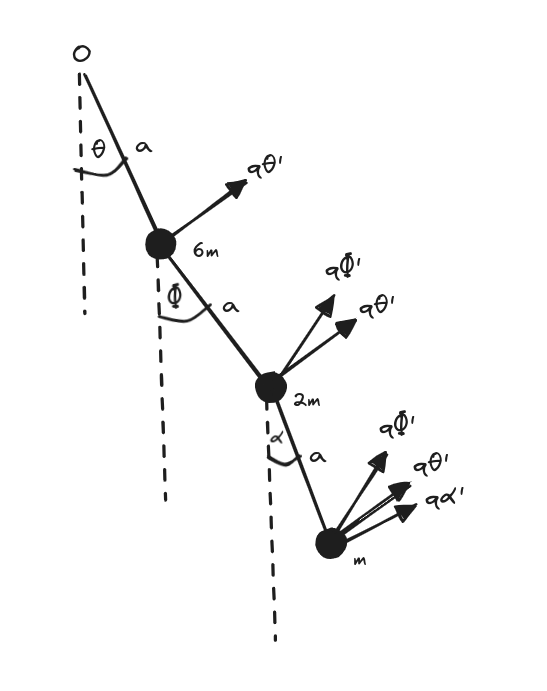
\includegraphics[scale=0.45]{ch15-4.png}
    \end{center}
    Then the kinetic energy of the system is given by
    \begin{align*}
        T &= \frac{1}{2}(6m)(a\bm{\dot\theta})^2
        + \frac{1}{2}(2m)a^2(\bm{\dot\theta} + \bm{\dot\phi})^2
        + \frac{1}{2}(m)a^2(\bm{\dot\theta} + \bm{\dot\phi} + \bm{\dot\alpha})^2\\
        &= 3ma^2\dot\theta^2
        + ma^2(\dot\theta^2 + \dot\phi^2 
        + 2\dot\theta\dot\phi\cos(\theta - \phi))\\
        &\quad+ \frac{1}{2}ma^2(\dot\theta^2 + \dot\phi^2 + \dot\alpha^2 
        + 2\dot\theta\dot\phi\cos(\theta - \phi)
        + 2\dot\theta\dot\alpha\cos(\theta - \alpha)\\
        &\quad + 2\dot\phi\dot\alpha\cos(\phi - \alpha))
    \end{align*}
    On the other hand, the potential energy is given by
    \begin{align*}
        V &= (6m + 2m + m)g a(1 - \cos\theta) 
        + (2m + m)g a(1 - \cos\phi)\\
        &\quad+ mga(1 - \cos\alpha)\\
        &= 9mga(1 - \cos\theta) + 3mga(1 - \cos\phi) + mga(1 - \cos\alpha)
    \end{align*}
    But for small oscillations about $\theta = \phi = \alpha = 0$
    we can approximate the equations for $T$ and $V$ as follows
    \begin{align*}
        T &= ma^2\left(3\dot\theta^2
        + \dot\theta^2 + \dot\phi^2 + 2\dot\theta\dot\phi
        + \frac{1}{2}(\dot\theta^2 + \dot\phi^2 + \dot\alpha^2 +
        2\dot\theta\dot\phi + 2\dot\theta\dot\alpha + 2\dot\phi\dot\alpha
        )\right)\\
        &= ma^2\left(\frac{9}{2}\dot\theta^2 + \frac{3}{2}\dot\phi^2
        + \frac{1}{2}\dot\alpha^2 + 3\dot\theta\dot\phi
        + \dot\theta\dot\alpha + \dot\phi\dot\alpha \right)
    \end{align*}
    and
    \begin{align*}
        V &= mga\left(\frac{9}{2}\theta^2 + \frac{3}{2}\phi^2
        + \frac{1}{2} \alpha^2\right)
    \end{align*}

    Then the $\bm{V}$-matrix and the $\bm{T}$-matrix are 
    \begin{align*}
        \bm{V} = mga\begin{pmatrix}
            9/2  & 0 & 0\\
            0 & 3/2 & 0\\
            0 & 0 & 1/2
        \end{pmatrix}\quad\quad
        \bm{T} = ma^2\begin{pmatrix}
            9/2  & 3/2 & 1/2\\
            3/2 & 3/2 & 1/2\\
            1/2 & 1/2 & 1/2
        \end{pmatrix}
    \end{align*}
    Now the determinant equation is given by
    \begin{align*}
        \det\begin{bmatrix}
            mga\begin{pmatrix}
                9/2  & 0 & 0\\
                0 & 3/2 & 0\\
                0 & 0 & 1/2
            \end{pmatrix}
            - ma^2\omega^2\begin{pmatrix}
                9/2  & 3/2 & 1/2\\
                3/2 & 3/2 & 1/2\\
                1/2 & 1/2 & 1/2
            \end{pmatrix} 
        \end{bmatrix} &= 0\\
        \det\begin{bmatrix}
            g \begin{pmatrix}
                9/2  & 0 & 0\\
                0 & 3/2 & 0\\
                0 & 0 & 1/2
            \end{pmatrix}
            - a\omega^2\begin{pmatrix}
                9/2  & 3/2 & 1/2\\
                3/2 & 3/2 & 1/2\\
                1/2 & 1/2 & 1/2
            \end{pmatrix}
        \end{bmatrix} &= 0\\
        \begin{vmatrix}
            (9/2)(g - a\omega^2) & - (3/2)a\omega^2 & -(1/2)a\omega^2\\
            - (3/2)a\omega^2 & (3/2)(g - a\omega^2) & -(1/2)a\omega^2\\
            -(1/2)a\omega^2 & -(1/2)a\omega^2 & (1/2)(g - a\omega^2)
        \end{vmatrix}
        &= 0\\
        \begin{vmatrix}
            (9/2)(1 - \mu) & - 3\mu/2 & -\mu/2\\
            - 3\mu/2 & (3/2)(1 - \mu) & -\mu/2\\
            -\mu/2 & -\mu/2 & (1/2)(1 - \mu)
        \end{vmatrix}
        &= 0\\
        ((27/8)(1 - \mu)^3 - 3\mu^3/8 - 3\mu^3/8)-\quad&\\
        (3\mu^2/8(1 - \mu) + 9\mu^2/8(1- \mu) + 9\mu^2/8 ( 1- \mu)) &= 0\\
        \frac{3}{8}\left(-11\mu^3 + 27\mu^2 - 27\mu + 9\right)
        - \frac{3}{8}\left(7\mu^2 - 7\mu^3\right)
        &= 0\\
        -4\mu^3 + 20\mu^2 - 27\mu + 9 &= 0\\
        12\mu^3 - 60\mu^2 + 81\mu - 27 &= 0
    \end{align*}
    Where in the last step we multiplied by $-3$ the equation.

    Knowing that the cubic equation has a root at $\mu = 3$ then dividing
    $12\mu^3 - 60\mu^2 + 81\mu - 27$ by $\mu - 3$ we get that
    $(\mu - 3)(12\mu^2 - 24\mu + 9) = 0$ hence the other two roots are
    $\mu = 1/2$ and $\mu = 3/2$. Therefore the normal frequencies are
    \begin{align*}
        \omega_1 = \sqrt{\frac{g}{2a}}\quad\quad
        \omega_2 = \sqrt{\frac{3g}{2a}}\quad\quad
        \omega_3 = \sqrt{\frac{3g}{a}}
    \end{align*}

    Now we want to determine the forms of the normal modes.
    To answer this we need to find the coordinate amplitudes in each of
    the normal modes.
    If the amplitudes of $\theta$, $\phi$ and $\alpha$ are $a_1$, $a_2$
    and $a_3$ respectively, then these amplitudes satisfy
    the following matrix equation
    \begin{align*}
        \begin{pmatrix}
            (9/2)(1 - \mu) & - 3\mu/2 & -\mu/2\\
            - 3\mu/2 & (3/2)(1 - \mu) & -\mu/2\\
            -\mu/2 & -\mu/2 & (1/2)(1 - \mu)
        \end{pmatrix}\cdot
        \begin{pmatrix}
            a_1\\ a_2 \\ a_3
        \end{pmatrix}
        &= 0
    \end{align*}    
    Then for the slow mode $\mu = 1/2$ we have that
    \begin{align*}
        \begin{pmatrix}
            9/4 & -3/4 & -1/4\\
            -3/4 & 3/4 & -1/4\\
            -1/4 & -1/4 & 1/4
        \end{pmatrix}\cdot
        \begin{pmatrix}
            a_1\\ a_2\\ a_3
        \end{pmatrix}
        &= 0\\
        \begin{pmatrix}
            9 & -3 & -1\\
            -3 & 3 & -1\\
            -1 & -1 & 1
        \end{pmatrix}\cdot
        \begin{pmatrix}
            a_1\\ a_2\\ a_3
        \end{pmatrix}
        &= 0
    \end{align*}
    From these equations, we have a family of non-trivial solutions
    $a_1 = \epsilon/3$, $a_2 = 2\epsilon/3$ and $a_3 = \epsilon$
    where $\epsilon$ can take any (non-zero) value. Setting $\epsilon = 3$
    we get that $\bm{a}_1 = (1, 2, 3)$.

    In the same way for $\mu = 3/2$ we have that
    \begin{align*}
        \begin{pmatrix}
            -9/4 & -9/4 & -3/4\\
            -9/4 & -3/4 & -3/4\\
            -3/4 & -3/4 & -1/4
        \end{pmatrix}\cdot
        \begin{pmatrix}
            a_1\\ a_2\\ a_3
        \end{pmatrix}
        &= 0\\
        \begin{pmatrix}
            9 & 9 & 3\\
            9 & 3 & 3\\
            3 & 3 & 1
        \end{pmatrix}\cdot
        \begin{pmatrix}
            a_1\\ a_2\\ a_3
        \end{pmatrix}
        &= 0
    \end{align*}
    From these equations, we have a family of non-trivial solutions
    $a_1 = \epsilon$, $a_2 = 0$ and $a_3 = -3\epsilon$
    where $\epsilon$ can take any (non-zero) value. Setting $\epsilon = 1$
    we get that $\bm{a}_2 = (1, 0, -3)$.

    Finally, for $\mu = 3$ we have that
    \begin{align*}
        \begin{pmatrix}
            9 & 9/2 & 3/2\\
            9/2 & 3 & 3/2\\
            3/2 & 3/2 & 1
        \end{pmatrix}\cdot
        \begin{pmatrix}
            a_1\\ a_2\\ a_3
        \end{pmatrix}
        &= 0
    \end{align*}
    From these equations, we have a family of non-trivial solutions
    $a_1 = \epsilon$, $a_2 = -3\epsilon$ and $a_3 = 3\epsilon$
    where $\epsilon$ can take any (non-zero) value. Setting $\epsilon = 1$
    we get that $\bm{a}_3 = (1, -3, 3)$.

    Lastly, we want to determine a set of normal coordinates.
    We already found that
    \begin{align*}
        \bm{T} = \frac{1}{2}ma^2\begin{pmatrix}
            9  & 3 & 1\\
            3 & 3 & 1\\
            1 & 1 & 1
        \end{pmatrix} \quad
        \bm{a}_1 = \begin{pmatrix}
            1 \\ 2 \\ 3
        \end{pmatrix}\quad
        \bm{a}_2 = \begin{pmatrix}
            1 \\ 0 \\ -3
        \end{pmatrix}\quad
        \bm{a}_1 = \begin{pmatrix}
            1 \\ -3 \\ 3
        \end{pmatrix}
    \end{align*}
    So a set of normal coordinates is given by
    \begin{align*}
        \eta_1 &= \begin{pmatrix}1 & 2 & 3\end{pmatrix}
        \cdot \begin{pmatrix}
            9  & 3 & 1\\
            3 & 3 & 1\\
            1 & 1 & 1
        \end{pmatrix}
        \cdot \begin{pmatrix}
            \theta \\ \phi \\ \alpha
        \end{pmatrix}
        = 6(3\theta + 2\phi + \alpha)\\
        %
        \eta_2 &= \begin{pmatrix}1 & 0 & -3\end{pmatrix}
        \cdot \begin{pmatrix}
            9  & 3 & 1\\
            3 & 3 & 1\\
            1 & 1 & 1
        \end{pmatrix}
        \cdot \begin{pmatrix}
            \theta \\ \phi \\ \alpha
        \end{pmatrix}
        = 2(3\theta -\alpha)\\
        %
        \eta_3 &= \begin{pmatrix}1 & -3 & 3\end{pmatrix}
        \cdot \begin{pmatrix}
            9  & 3 & 1\\
            3 & 3 & 1\\
            1 & 1 & 1
        \end{pmatrix}
        \cdot \begin{pmatrix}
            \theta \\ \phi \\ \alpha
        \end{pmatrix}
        = 3\theta - 3\phi  + \alpha
    \end{align*}
\end{proof}
\begin{proof}{\textbf{15.9}}
    The system in this case looks like the following 
    \begin{center}
        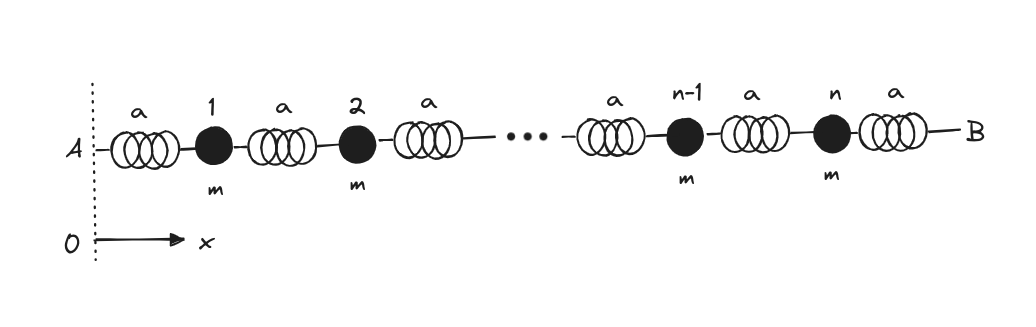
\includegraphics[scale=0.4]{ch15-9.png}
    \end{center}
    Where each mass is a distance $a$ apart and the distance from $A$
    to $B$ is $(n+1)a$. Each mass has an equilibrium point at $x=ia$,
    let us suppose each mass now has a displacement from the equilibrium
    point given by $x_i$ where $i=1,...,n$ then we have that
    \begin{align*}
        T = T^{app} &= \frac{1}{2}m\dot{x}_1^2 + \frac{1}{2}m\dot{x}_2^2 +
        ... + \frac{1}{2}m\dot{x}_n^2\\
        V = V^{app} &= \frac{1}{2}\alpha x_1^2 +
        \frac{1}{2}\alpha(x_2 - x_1)^2 + \frac{1}{2}\alpha(x_3 - x_2)^2 + ...\\
        &\quad... + \frac{1}{2}\alpha(x_n - x_{n-1})^2 + \frac{1}{2}\alpha x_n^2\\
        &= \frac{1}{2}\alpha(
            x_1^2 + x_1^2 -2x_1 x_2 + x_2^2 + x_3^2 -2x_3 x_2 + x_2^2 +\\
            &\quad... + x_n^2 -2x_nx_{n-1} +x_{n-1}^2 + x_n^2)\\
        &= \frac{1}{2}\alpha(
            2x_1^2 + 2x_2^2 + 2x_3^2 + ... + 2x_{n-1}^2 + 2x_n^2\\
            &\quad -2x_1 x_2 -2x_3 x_2 + ... -2x_nx_{n-1} )
    \end{align*}
    Then the $\bm{V}$-matrix and the $\bm{T}$-matrix are 
    \begin{align*}
        \bm{T} = \frac{1}{2}m\begin{pmatrix}
            1  & 0 & 0 &... & 0\\
            0 & 1 & 0 &... & 0\\
            \vdots & \vdots & \vdots & \vdots & \vdots\\
            0 & 0 & 0 &... & 1
        \end{pmatrix}
        \quad\quad
        \bm{V} = \frac{1}{2}\alpha\begin{pmatrix}
            2  & -1 & 0 &... & 0\\
            -1 & 2 & -1 &... & 0\\
            \vdots & \vdots & \vdots & \vdots & \vdots\\
            0 & 0 & 0 &... & 2          
        \end{pmatrix}
    \end{align*}
    Now the determinantal equation is given by
    \begin{align*}
        \begin{vmatrix}
            \frac{1}{2}\alpha\begin{pmatrix}
                2  & -1 & 0 &... & 0\\
                -1 & 2 & -1 &... & 0\\
                \vdots & \vdots & \vdots & \vdots & \vdots\\
                0 & 0 & 0 &... & 2    
            \end{pmatrix}
            - \frac{1}{2}\omega^2m\begin{pmatrix}
                1  & 0 & 0 &... & 0\\
                0 & 1 & 0 &... & 0\\
                \vdots & \vdots & \vdots & \vdots & \vdots\\
                0 & 0 & 0 &... & 1
            \end{pmatrix}
        \end{vmatrix} &= 0\\
        \begin{vmatrix}
                (2\alpha - \omega^2m)  & -\alpha & 0 &... & 0\\
                -\alpha & (2\alpha - \omega^2m) & -\alpha &... & 0\\
                \vdots & \vdots & \vdots & \vdots & \vdots\\
                0 & 0 & 0 & ... & (2\alpha - \omega^2m)
        \end{vmatrix} &= 0\\
        \begin{vmatrix}
            2\alpha(1 - \omega^2m/2\alpha)  & -\alpha & 0 &... & 0\\
            -\alpha & 2\alpha(1 - \omega^2m/2\alpha) & -\alpha &... & 0\\
            \vdots & \vdots & \vdots & \vdots & \vdots\\
            0 & 0 & 0 &... & 2\alpha(1 - \omega^2m/2\alpha)
    \end{vmatrix} &= 0
    \end{align*}
    Let us set $\cos\theta = 1 - (\omega^2m/2\alpha)$ then we get that
    \begin{align*}
        \Delta_n = \begin{vmatrix}
            2\cos\theta  & -1 & 0 & ... & 0\\
            -1 & 2\cos\theta & -1 & ... & 0\\
            \vdots & \vdots & \vdots & \vdots & \vdots\\
            0 & 0 & 0 &... & 2\cos\theta
    \end{vmatrix} &= 0
    \end{align*}
    By expanding the determinant by the top row we have that
    \begin{align*}
        \Delta_{n} = 2\cos\theta\Delta_{n-1} + (-1)(-1)^3\begin{vmatrix}
        -1 & -1 & 0 &... & 0\\
        0 & 2\cos\theta& -1 & ... & 0\\
        \vdots & \vdots & \vdots & \vdots & \vdots\\
        0 & 0 & 0 &... & 2\cos\theta
    \end{vmatrix}
    \end{align*}
    Hence, by expanding the last determinant by the first column we have that
    \begin{align*}
        \Delta_{n} = 2\cos\theta\Delta_{n-1} -\Delta_{n-2}
    \end{align*}
    Now, let us apply induction to show that
    $\sin((n+1)\theta)/\sin\theta = \Delta_n$.
    In the base case for $n = 1$ we see that
    \begin{align*}
        \frac{\sin(2\theta)}{\sin\theta}
        = \frac{2\cos\theta\sin\theta}{\sin\theta}
        = 2\cos\theta = \Delta_1
    \end{align*}
    Suppose that $\Delta_{n-1} = \sin n\theta/\sin\theta$ is true then
    \begin{align*}
        \frac{\sin((n +1)\theta)}{\sin\theta}
        &= \frac{\sin((n + 1)\theta) + \sin((n - 1)\theta)
        - \sin((n - 1)\theta)}{\sin\theta}\\
        &= \frac{\sin n\theta\cos\theta + \cos n\theta\sin\theta
        + \sin(n\theta)\cos\theta - \cos n\theta\sin\theta}
        {\sin\theta} - \Delta_{n-2}\\
        &= \frac{2\sin n\theta\cos\theta}{\sin\theta} - \Delta_{n-2}\\
        &= 2\cos\theta\Delta_{n-1} - \Delta_{n-2}\\
        &= \Delta_n
    \end{align*}
    Therefore it's shown by induction that
    $\Delta_n = \sin((n+1)\theta)/\sin\theta$.

    Finally, we want to deduce the normal frequencies of the system so we need
    to solve the equation $\Delta_n = 0$ i.e.
    $$\frac{\sin((n+1)\theta)}{\sin\theta} = 0$$
    And this will happen when
    \begin{align*}
        (n+1)\theta = i\pi
    \end{align*}
    for $i = 0,1,2,...$, hence
    \begin{align*}
        % \theta &= \frac{i\pi}{n+1}\\
        \cos\theta &= \cos\bigg(\frac{i\pi}{n+1}\bigg)\\
        1 - \frac{\omega_i^2m}{2\alpha} &= \cos\bigg(\frac{i\pi}{n+1}\bigg)\\
        \omega_i &= \sqrt{\frac{2\alpha}{m}\bigg(1 - \cos\bigg(\frac{i\pi}{n+1}\bigg)\bigg)}\\
        \omega_i &= \sqrt{\frac{2\alpha}{m}}
        \sqrt{\frac{2\bigg(1 - \cos\bigg(\frac{i\pi}{n+1}\bigg)\bigg)}{2}}\\
        \omega_i &= 2\sqrt{\frac{\alpha}{m}}\sin\bigg(\frac{i\pi}{2(n+1)}\bigg)
    \end{align*}
    Where we used that $\sin(\gamma/2) = \sqrt{(1- \cos\gamma)/2}$.
\end{proof}
\cleardoublepage
\begin{proof}{\textbf{15.11}}
    The system in this case looks like the following 
    \begin{center}
        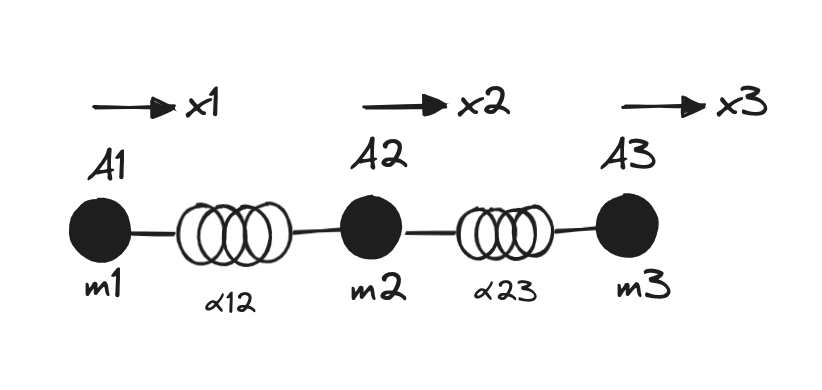
\includegraphics[scale=0.45]{ch15-11.png}
    \end{center}
    Let the displacement of the three atoms from their equilibrium positions
    be $x_1, x_2, x_3$ in the positive direction (to the right)
    then we have that
    \begin{align*}
        T = T^{app} &= \frac{1}{2}m_1\dot{x}_1^2 + \frac{1}{2}m_2\dot{x}_2^2 +
        \frac{1}{2}m_3\dot{x}_3^2\\
        V = V^{app} &=
        \frac{1}{2}\alpha_{12}(x_2 - x_1)^2 + \frac{1}{2}\alpha_{23}(x_3 - x_2)^2\\
        &= \frac{1}{2}\alpha_{12}(x_1^2 - 2x_1x_2 + x_2^2) + 
        \frac{1}{2}\alpha_{23}(x_2^2 - 2x_2x_3 + x_3^2)\\
        &= \frac{1}{2}(\alpha_{12}x_1^2 - 2\alpha_{12}x_1x_2 + 
        (\alpha_{12} + \alpha_{23})x_2^2 - 2\alpha_{23}x_2x_3 + \alpha_{23}x_3^3)
    \end{align*}
    Then the $\bm{V}$-matrix and the $\bm{T}$-matrix are 
    \begin{align*}
        \bm{T} = \frac{1}{2}\begin{pmatrix}
            m_1 & 0 & 0 \\
            0 & m_2 & 0 \\
            0 & 0 & m_3
        \end{pmatrix}
        \quad\quad
        \bm{V} = \frac{1}{2}\begin{pmatrix}
            \alpha_{12} & -\alpha_{12} & 0\\
            -\alpha_{12} & (\alpha_{12} + \alpha_{23}) & -\alpha_{23}\\
            0 & -\alpha_{23} & \alpha_{23}
        \end{pmatrix}
    \end{align*}
    Now the determinantal equation is given by
    \begin{align*}
        \begin{vmatrix}
            \frac{1}{2}\begin{pmatrix}
                \alpha_{12} & -\alpha_{12} & 0\\
                -\alpha_{12} & (\alpha_{12} + \alpha_{23}) & -\alpha_{23}\\
                0 & -\alpha_{23} & \alpha_{23}
            \end{pmatrix}
            - \frac{1}{2}\omega^2\begin{pmatrix}
                m_1 & 0 & 0 \\
                0 & m_2 & 0 \\
                0 & 0 & m_3
            \end{pmatrix}
        \end{vmatrix} &= 0\\
        \begin{vmatrix}
                (\alpha_{12} - \omega^2m_1)  & -\alpha_{12} & 0 \\
                -\alpha_{12} & (\alpha_{12} + \alpha_{23} - \omega^2m_2) & -\alpha_{23} \\
                0 & -\alpha_{23} & (\alpha_{23} -\omega^2 m_3)
        \end{vmatrix} &= 0\\
        (\alpha_{12} - \omega^2m_1)(\alpha_{12} + \alpha_{23} - \omega^2m_2)(\alpha_{23} -\omega^2 m_3)\\
        - \alpha_{12}^2(\alpha_{23} -\omega^2 m_3)
        - \alpha_{23}^2(\alpha_{12} - \omega^2m_1) 
        &= 0\\
        (\alpha_{12}^2 + \alpha_{12}\alpha_{23} - \alpha_{12}\omega^2(m_1 + m_2)
        - \alpha_{23}\omega^2m_1 + \omega^4m_1m_2)
        (\alpha_{23} -\omega^2 m_3)\\
        - \alpha_{12}^2(\alpha_{23} -\omega^2 m_3)
        - \alpha_{23}^2(\alpha_{12} - \omega^2m_1) &= 0\\
        %
        (\alpha_{12}\alpha_{23} - \alpha_{12}\omega^2(m_1 + m_2)
        - \alpha_{23}\omega^2m_1 + \omega^4m_1m_2)
        (\alpha_{23} -\omega^2 m_3)\\
        - \alpha_{23}^2(\alpha_{12} - \omega^2m_1) &= 0\\
        %
        \alpha_{12}\alpha_{23}^2 - \alpha_{12}\alpha_{23}\omega^2(m_1 + m_2)
        - \alpha_{23}^2\omega^2m_1 + \alpha_{23}\omega^4m_1m_2\\
        -\alpha_{12}\alpha_{23}\omega^2 m_3
        + \alpha_{12}\omega^4m_3(m_1 + m_2)
        + \alpha_{23}\omega^4m_1m_3 - \omega^6m_1m_2m_3\\
        - \alpha_{23}^2\alpha_{12} + \alpha_{23}^2\omega^2m_1 &= 0\\
        %
        - \alpha_{12}\alpha_{23}(m_1 + m_2)
         + \alpha_{23}\omega^2m_1m_2
        -\alpha_{12}\alpha_{23} m_3\\
        + \alpha_{12}\omega^2m_3(m_1 + m_2)
        + \alpha_{23}\omega^2m_1m_3 - \omega^4m_1m_2m_3 
        &= 0\\
        \omega^4m_1m_2m_3
        - [\alpha_{12}m_3(m_1 + m_2) + \alpha_{23}m_1(m_2 + m_3)]\omega^2\\
        + \alpha_{12}\alpha_{23}(m_1 + m_2 + m_3)
        &= 0
    \end{align*}
    In the case where $m_1 = 3m$, $m_2 = m$, $m_3 = 2m$ and
    $\alpha_{12} = 3\alpha$, $\alpha_{23} = 2 \alpha$ the determinantal
    equation becomes
    \begin{align*}
        6\omega^4m^3 - [6\alpha m(3m + m) + 6\alpha m(m + 2m)]\omega^2
        + 6\alpha^2(3m + m + 2m) &= 0\\
        \omega^4m^2 - 7\alpha m\omega^2 + 6\alpha^2 &= 0
    \end{align*}
    Solving this 2nd-degree equation in terms of $\omega^2$
    we get the vibrational frequencies as follows
    \begin{align*}
        \omega_1^2 &=
            \frac{7\alpha m - \sqrt{49\alpha^2 m^2 - 24m^2\alpha^2}}{2m^2}
            = \frac{7\alpha m - 5\alpha m}{2m^2}
            = \frac{\alpha}{m}\\
        \omega_2^2 &=
        \frac{7\alpha m + \sqrt{49\alpha^2 m^2 - 24m^2\alpha^2}}{2m^2}
            = \frac{7\alpha m + 5\alpha m}{2m^2}
            = \frac{6\alpha}{m}
    \end{align*}
    According to Table 2 we can estimate the ratio of vibrational frequencies
    for the molecule $OCS$ by taking the values of $\lambda_1^{-1}$
    for the molecules $CO_2$ and $CS_2$ and computing the ratio between them
    in this way we get a value of $2.03$.
    The frequency ratio we can compute with the equations we got gives us
    $\omega_2/\omega_1 = \sqrt{6} = 2.45$ which is closer than the estimation
    to the ratio measured for the molecule $OCS$ which is $2.49$.
\end{proof}
\cleardoublepage
\begin{proof}{\textbf{15.14}}
    Let us consider the symmetric motion of the molecule as shown below
    \begin{center}
        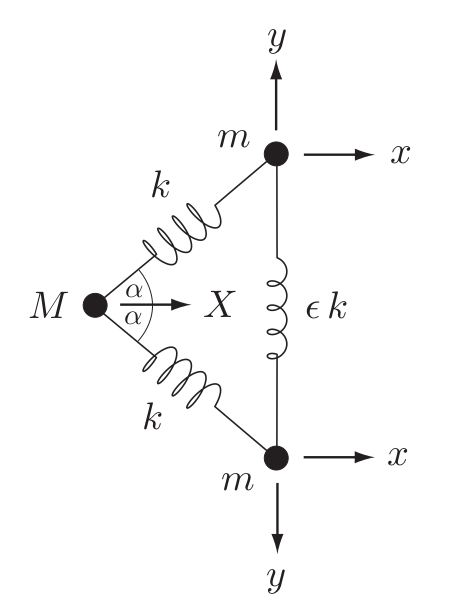
\includegraphics[scale=0.45]{ch15-14.png}
    \end{center}
    In this case, we are considering the special case in which $M = 2m$ and
    $\alpha = 60^\circ$. Then the approximated kinetic energy is given by
    \begin{align*}
        T = T^{app} &= \frac{1}{2}m(\bm{\dot{x}} + \bm{\dot{y}})^2
        + \frac{1}{2}m(\bm{\dot{x}} + \bm{\dot{y}})^2 + m\bm{\dot{X}}^2\\
            &= \frac{1}{2}m(\dot{x}^2 + \dot{y}^2)
        + \frac{1}{2}m(\dot{x}^2 + \dot{y}^2) + m\dot{X}^2
    \end{align*}
    But for the potential energy let us note that if $r$ is the relaxed length
    of both the springs between $M$ and $m$ then the length after
    the displacements $X, x, y$ is
    $\sqrt{(r\cos\alpha + x - X)^2 + (r\sin\alpha + y)^2}$.
    So the difference between these lengths
    only taking the non-quadratic terms involving $x,X$, and $y$ is
    \begin{align*}
        &\sqrt{(r\cos\alpha + x - X)^2 + (r\sin\alpha + y)^2} - r =\\
        &\qquad=
        \sqrt{r^2\cos^2\alpha + 2rx\cos\alpha - 2rX\cos\alpha + 
        r^2\sin^2\alpha + 2ry\sin\alpha} - r\\
        &\qquad=
        \sqrt{r^2(\cos^2\alpha + \sin^2\alpha) + 2r(x\cos\alpha
        - X\cos\alpha + y\sin\alpha)} - r\\
        &\qquad=
        r\sqrt{1 + \frac{2(x\cos\alpha - X\cos\alpha + y\sin\alpha)}{r}} - r\\
        &\qquad=
        r\bigg(1 + \frac{(x\cos\alpha - X\cos\alpha + y\sin\alpha)}{r}\bigg) - r\\
        &\qquad= x\cos\alpha - X\cos\alpha + y\sin\alpha
    \end{align*}
    Where we also used the binomial approximation applied to the square root.
    Then the approximated potential energy is
    \begin{align*}
        V = V^{app} &= \frac{1}{2}k(x\cos\alpha - X\cos\alpha + y\sin\alpha)^2 +\\
        &\quad+ \frac{1}{2}k(x\cos\alpha - X\cos\alpha + y\sin\alpha)^2
        + \frac{1}{2}\epsilon k(2y)^2\\
        &= k(x^2\cos^2\alpha - 2xX\cos^2\alpha + X^2\cos^2\alpha + \\
        &\quad + 2xy\cos\alpha\sin\alpha - 2Xy\cos\alpha\sin\alpha +
        y^2(\sin^2\alpha + 2\epsilon))
    \end{align*}
    This implies that the $\bm{V}$-matrix and the $\bm{T}$-matrix are 
    \begin{align*}
        \bm{T} = m\begin{pmatrix}
            1 & 0 & 0 \\
            0 & 1 & 0 \\
            0 & 0 & 1
        \end{pmatrix}
        \quad\quad
        \bm{V} = k\begin{pmatrix}
            \cos^2\alpha & -\cos^2\alpha & \cos\alpha\sin\alpha\\
            -\cos^2\alpha & \cos^2\alpha & -\cos\alpha\sin\alpha\\
            \cos\alpha\sin\alpha & -\cos\alpha\sin\alpha & \sin^2\alpha + 2\epsilon
        \end{pmatrix}
    \end{align*}
    Now the determinantal equation is given by
    \begin{align*}
        \begin{vmatrix}
            k\begin{pmatrix}
                \cos^2\alpha & -\cos^2\alpha & \cos\alpha\sin\alpha\\
                -\cos^2\alpha & \cos^2\alpha & -\cos\alpha\sin\alpha\\
                \cos\alpha\sin\alpha & -\cos\alpha\sin\alpha &
                \sin^2\alpha + 2\epsilon
            \end{pmatrix}
            - m\omega^2\begin{pmatrix}
                1 & 0 & 0 \\
                0 & 1 & 0 \\
                0 & 0 & 1
            \end{pmatrix}
        \end{vmatrix} &= 0
    \end{align*}
    And using that $\mu = \frac{m\omega^2}{k}$ we have that
    \begin{align*}
        \begin{vmatrix}
            \begin{pmatrix}
                \cos^2\alpha & -\cos^2\alpha & \cos\alpha\sin\alpha\\
                -\cos^2\alpha & \cos^2\alpha & -\cos\alpha\sin\alpha\\
                \cos\alpha\sin\alpha & -\cos\alpha\sin\alpha &
                \sin^2\alpha + 2\epsilon
            \end{pmatrix}
            - \mu\begin{pmatrix}
                1 & 0 & 0 \\
                0 & 1 & 0 \\
                0 & 0 & 1
            \end{pmatrix}
        \end{vmatrix} &= 0\\
        \begin{vmatrix}
            \cos^2\alpha - \mu & -\cos^2\alpha & \cos\alpha\sin\alpha\\
            -\cos^2\alpha & \cos^2\alpha - \mu & -\cos\alpha\sin\alpha\\
            \cos\alpha\sin\alpha & -\cos\alpha\sin\alpha &
            \sin^2\alpha + 2\epsilon - \mu
        \end{vmatrix} &= 0\\
        % {{cos^2(a) - mu, -cos^2(a), cos(a)sin(a)},{-cos^2(a), cos^2(a)- mu, -cos(a)sin(a)},{cos(a)sin(a), -cos(a)sin(a), sin^2(a) + 2epsilon - mu}}
        \mu (\mu (\sin^2(\alpha) - \mu + 2\epsilon)
        + \cos^2(\alpha) (2\mu - 4\epsilon))&= 0\\
        \frac{3}{4}\mu - \mu^2 + 2\mu\epsilon
        + \frac{1}{2}\mu - \epsilon &= 0\\
        - \mu^2 + \mu(\frac{5}{4} + 2\epsilon) - \epsilon &= 0\\
        4\mu^2 - \mu(5 + 8\epsilon) + 4\epsilon &= 0
    \end{align*}
    Where in the last step we multiplied the whole equation by $-4$.

    Finally, we solve the equation to compute the vibrational frequencies
    ratio
    \begin{align*}
        \mu_1 = \frac{(5 + 8\epsilon) - \sqrt{25 + 16\epsilon + 64\epsilon^2}}
        {8}\\
        \mu_2 = \frac{(5 + 8\epsilon) + \sqrt{25 + 16\epsilon + 64\epsilon^2}}
        {8}
    \end{align*}
    Then the ratio between $\mu_2$ and $\mu_1$ gives us the vibrational
    frequencies ratio as follows
    \begin{align*}
        \frac{m\omega_2^2/k}{m\omega_1^2/k} = \frac{\omega_2^2}{\omega_1^2}
        = \frac{(5 + 8\epsilon) + \sqrt{25 + 16\epsilon + 64\epsilon^2}}
        {(5 + 8\epsilon) - \sqrt{25 + 16\epsilon + 64\epsilon^2}}
    \end{align*}
    According to the data we have sulphur dioxide has a ratio of
    $\lambda_2^{-1} /\lambda_1^{-1} = 525/1151$
    so the value of epsilon should be such that
    \begin{align*}
        (5 + 8\epsilon) + \sqrt{25 + 16\epsilon + 64\epsilon^2} = 525\\
        (5 + 8\epsilon) - \sqrt{25 + 16\epsilon + 64\epsilon^2} = 1151
    \end{align*}
    So adding both equations we have that
    \begin{align*}
        2(5 + 8\epsilon) &= 1676\\
        \epsilon &= \frac{838 -5}{8}\\
        \epsilon &= 104.25
    \end{align*}
    This implies that we need an $\epsilon > 1$ but we started with
    the assumption that $\epsilon$ was a small number, therefore there is no
    $\epsilon$ such that we match the measured ratio.
\end{proof}












\end{document}



















